\chapter{Introduction} \label{ch:introduction}

\dictum{%
   Provably optimal and heuristically fast.}
\vskip 1em

\graphicspath{{\dir/}}

% The problem looked strange to work on; I didn't believe nobody has done it
% before
%\section{Research goals and scope}
%\paragraph{Problem statement}
%\paragraph{Problem domain}
%only optimal alignment in this thesis
%asymptotics analysis

\section{Alignment problem}

% Sequencing and variant calling
The analysis and understanding of genetic variation encoded in the genome of an
organism lies at the center of computational biology and medicine. Variation is
usually identified through matching sequences obtained from DNA/RNA-sequencing
back to a reference (genome) sequence in the process of \emph{variant calling},
making the alignment task a core problem in sequence bioinformatics.

% paper:seeds
\subsection{Problem statement: Alignment as shortest path} \label{SEEDsec:task}
%
In the following, we formalize the task of optimally aligning a read to a
reference graph in terms of finding a shortest path in an \emph{alignment
graph}. Our discussion closely follows~\citep{ivanov2020astarix} and is in line
with~\citep{rautiainen_aligning_2017}.

\para{Reference graph}
%
A reference graph $\RG=(\RGV,\RGE)$ encodes a collection of references to be
considered when aligning a read. Its directed edges $\RGE \subseteq \RGV \times
\RGV \times \Sigma$ are labeled by nucleotide letters from $\Sigma =
\{\texttt{A},\texttt{C},\texttt{G},\texttt{T}\}$, hence any walk
$\reference{\pi}$ in $\RG$ spells a string $\sigma(\reference{\pi}) \in
\Sigma^*$.

An alignment of a read $q \in \Sigma^*$ to a reference graph $\RG$ consists of
(i)~a walk $\reference{\pi}$ in $\RG$ and (ii)~a sequence of edits (matches,
substitutions, deletions, and insertions) that transform
$\sigma(\reference{\pi})$ to $q$. An alignment is \emph{optimal} if it minimizes
the sum of edit costs for a given real-valued cost model $\cedits = (\cmatch,
\csubst,\cdel, \cins)$.
%
We assume that edit costs are non-negative---a pre-requisite for the correctness
of \A. Further, we assume that $\cmatch \leq \csubst, \cins, \cdel$---a
prerequisite for the correctness of our heuristic.

We note that our approach naturally works for cyclic reference graphs.

\begin{figure}[t]
	\begin{alignat*}{20}
		(
			&\langle&& u &,& i   &\rangle&,
			&\langle&  v &,& i+1 &\rangle&,
			&&q[i],
			&&\cmatch
		&)&\in \AGE
		&& \quad \text{ if } (u,v,\ell) \in \RGE, \ell = q[i] & \qquad \text{(match)}\\
		%
		(
			&\langle&& u &,& i   &\rangle&,
			&\langle&  v &,& i+1 &\rangle&,
			&&q[i],
			&&\csubst
		&) &\in \AGE
		&& \quad \text{ if } (u,v,\ell) \in \RGE, \ell \neq q[i] & \qquad \text{(substitution)}\\
		%
		(
			&\langle&& u &,& i &\rangle&,
			&\langle&  v &,& i &\rangle&,
			&&\varepsilon,
			&&\cdel
		&) &\in \AGE
		&& \quad \text{ if } (u,v,\ell) \in \RGE & \qquad \text{(deletion)}\\
		%
		(
			&\langle&& u &,& i   &\rangle&,
			&\langle&  u &,& i+1 &\rangle&,
			&&q[i],
			&&\cins
		&) &\in \AGE
		&& \quad & \qquad \text{(insertion)},
	\end{alignat*}
	\caption[Formal definition of alignment graph]{Formal definition of
	alignment graph edges $\AGE \subseteq \AGV[q] \times \AGV[q] \times
	\Sigma_\varepsilon \times \mathbb{R}_{\geq 0}$. Here, $u,v \in \RGV$, $0
	\leq i < |q|$, $\ell \in \Sigma$, and $\varepsilon$ represents the empty
	string, indicating that letter $\ell$ was deleted.}
	\label{SEEDfig:graph-edges}
\end{figure}

\para{Alignment graph}
%
In order to formalize optimal alignment as a shortest path finding problem, we
rely on an \emph{alignment graph} $\AG[q]=(\AGV[q],\AGE[q])$.
%
Its nodes $\AGV[q]$ are \emph{states} of the form $\langle v, i \rangle$, where
$v \in \RGV$ is a node in the reference graph and $i \in \{0, \dots, |q|\}$
corresponds to a position in the read $q$.
%
Its edges $\AGE[q]$ are selected such that any path $\alignment{}{\pi}$ in
$\AG[q]$ from $\langle u, 0 \rangle$ to $\langle v, i \rangle$ corresponds to an
alignment of the first $i$ letters of $q$ to $\RG$.
%
Further, the edges are weighted, which allows us to define an \emph{optimal
alignment} of a read $q \in \Sigma^*$ as a shortest path $\alignment{}{\pi}$ in
$\AG[q]$ from $\langle u, 0 \rangle$ to $\langle v, |q| \rangle$, for any $u, v
\in \RGV$.
%
\cref{SEEDfig:graph-edges} formally defines the edges $\AGE$.

% paper:global
\paragraph{Sequences}
The input sequences $A = \overline{a_0a_1\dots a_i \dots a_{n-1}}$ and $B =
\overline{b_0b_1 \dots b_j \dots b_{m-1}}$ are over an alphabet $\Sigma$ with
$4$ letters. We refer to substrings $\overline{a_i \dots a_{i'-1}}$ as
$\substr Ai{i'}$, to prefixes $\overline{a_0 \dots a_{i-1}}$ as $A_{<i}$, and to
suffixes $\overline{a_i \dots a_{n-1}}$ as $A_{\geq i}$. The \emph{edit
distance} $\ed(A,B)$ is the minimum number of insertions, deletions, and
substitutions of single letters needed to convert $A$ into $B$.

\paragraph{Edit graph}
Let \emph{state} $\st{i}{j}$ denote the subtask of aligning the prefix $A_{<i}$
to the prefix $B_{<j}$. The \emph{edit graph} (also called \emph{alignment
graph}) $G(V,E)$ is a weighted directed graph with vertices $V = \{\st ij \vert
{0\leq i \leq n}, {0\leq j\leq m}\}$ corresponding to all states, and edges
connecting tasks to subtasks: edge ${\st ij \to \st{i{+}1}{j{+}1}}$ has cost
$0$ if ${a_i = b_j}$ (match) and $1$ otherwise (substitution), and edges ${\st ij
\to \st{i{+}1}{j}}$ (deletion) and ${\st ij \to\st{i}{j{+}1}}$ (insertion) have cost
$1$. We denote the root state $\st 00$ by $v_s$ and the target state $\st nm$ by
$v_t$.
For brevity we write $f(\st ij)$ as $f \st ij$.
The edit graph is a natural representation of the alignment problem that
provides a base for all alignment algorithms.
\section{Motivation}

Observation 1: A long query has more information that may hint towards the best
alignment place. Unlike the practical approximate algorithms, the existing optimal
algorithm do not exploit this information. As a result, all state-of-the-art
optimal algorithms take longer to map a longer query to a reference. 

Observation 2: The input is linear, the output is linear, the best case is
linear. On the other hand all optimal solutions are near-quadratic and the
theoretical limit is near-quadratic. To spead up beyond this near-quadratic
barrier, current practical algorithms break the optimality guarantee hoping that
the produced alignments are accurate enough. 

%But it is possible to be fast and accurate in the same time?
We take another approach: we preserve the optimality guarantee and use
substantially more information with the hope to be fast enough. As it turns out,
when the error rate is limited, our optimal solutions empirically scale
near-linearly up to very long sequences. This translates to many orders of
magnitude of runtime speedup compared to state-of-the-art optimal aligners.

% Problem, applications
The problem of aligning one biological sequence to another has been formulated
over half a century ago~\citep{needleman1970general} and is known as
\emph{global pairwise alignment}~\citep{navarro2001guided}. Pairwise alignment
has numerous applications in computational biology, such as genome assembly,
read alignment, variant detection, multiple sequence alignment, and differential
expression~\citep{prjibelski2018sequence}. Despite the centrality and age of
pairwise alignment, ``a major open problem is to implement an algorithm with linear-like
empirical scaling on inputs where the edit distance is linear
in~$n$''~\citep{medvedev2022theoretical}.

% Near-quadratic worst case
Alignment accuracy affects the subsequent analyses, so a common goal
is to find a shortest sequence of edit operations (insertions, deletions, and
substitutions of single letters) that transforms one sequence into the other.
Finding such a sequence of operations is at least as hard as computing the \emph{edit
distance}, which has recently been proven to not be computable in strongly
subquadratic time, unless SETH is false~\citep{backurs2015edit}. Given that
the number of sequencing errors is proportional to the length, existing exact aligners are
limited by quadratic scaling not only in the worst case but also in practice.
This is a computational bottleneck given the growing amounts of biological data
and the increasing sequence lengths~\citep{kucherov2019evolution}.

Sequence alignment is a class of combinatorial problems that is of primary
importance for analysis of genetic data. Algorithms and tools for alignment have
been thoroughly developed and routinely used for genome assembly, RNA
quantification, detecting splicing, oncology, multiple sequence alignment (MSA),
and evolutionary biology. Types of sequence alignment include global alignment,
semi-global alignment, alignment, local alignment, and others. For each type, a
common tradeoff that had to be done is between the alignment accuracy and the
performance to find it.

% graph reference
An additional difficulty is the fact that in the
upcoming pangenomic era, these algorithms must be also applicable to complex
graph structures. For more than 60 years, a linear sequence has been extremely
useful as a representation of a single genome. The affordability of sequencing
technologies enables not only to sequence genomes deeper but also to sequence
many genomes (e.g. of organisms or single cells), building a pangenome (an
abstracted genome that represents the genetic variation of a whole clade). The
shift towards population studies in the last decade motivates the adoption of
graph data structures which serve as compressed representations of collections
of related genomes (genomes are paths in the graph).

% \A context 
An optimal alignment can naturally be represented as a shortest path in an
alignment graph (equivalent to the DP table). In order to find such a shortest
path with minimal exploration, we instantiate the \A algorithm with a novel
heuristic function based on the unaligned parts of the sequences. This
additional information is a problem-specific heuristic function and it heavily
determines the efficiency of the search. For any explored state by \A, this
heuristic function should compute a lower bound on the remaining path length, or
more specifically, the minimal cost of edit operations needed to align the
remaining sequences.

%only optimal alignment in this thesis
%asymptotics analysis
%????? linear I/O but quadratic optimal

% Accuracy and Metrics
The number of possible ways that two sequence can be aligned grow exponentially
with length. The usual underlying question to finding ``correct'' alignments.
Regarding the precision of alignment, one is usually interested in base-to-base
(aka letter-to-letter) correspondence between the sequences, even though for
some applications a less detailed solution is sufficient: only the similarity
between sequences or the location where a read maps to a reference. Exact
alignment is only useful for very short sequences (often kmers), and for all
other cases the optimized metric may be hamming distance, edit distance (unit
costs), Levenshtein distance, affine costs, convex and concave costs, general
costs and others. 

% Problem statement
Depending on the the number of aligned sequences, there is pairwise alignment
and multiple sequence alignment (MSA). Depending on the parts of the sequences
that are aligned to each other, we differentiate global, local and various
semi-global alignemnts. There are generalizations to sequence-to-sequence
alignment, including aligning to nonlinear structures, such as directed acyclic
graphs, DAGs, general graphs and others. These structures are nowadays becoming
more common as a compressed form of representing a set of references to which a
sequence can be aligned. Often, one best alignment is suefficient but finding
several best (top-K) alignments. In the context of read alignment, a set of reads
is aligned to the same reference sequence so an indexing procedure is often
useful for the performance.

We specifically consider the alignment of a set of reads to a general graph, and
the global pairwise alignment.

Existing optimal algorithms are based on dynamic programming (DP) and
run in quadratic time (assuming that the number of errors is proportional to the
length)

we employ the \A algorithm which is an \emph{informed search} algorithm.
TODO: a case for the informed algorithms

% Heuristics for alignment
Both for sequence-to-sequence alignment and sequence-to-graph alignment,
heuristics are employed to keep alignment
tractable~\cite{altschul_basic_1990,langmead_fast_2012,garrison_variation_2018},
especially for large populations of human-sized genomes.
%
% Importance of optimal alignment
While such heuristics find the correct alignment for simple references, they
often perform poorly in regions of very high complexity, such as in the human
major histocompatibility complex (MHC)~\cite{dilthey_improved_2015}, in complex
but rare genotypes arising from somatic-subclones in tumor sequencing
data~\cite{harismendy_detection_2011}, or in the presence of frequent sequencing
errors~\cite{salmela_lordec_2014}.
%
Importantly, these cases can be of specific clinical or biological interest, and
incorrect alignment can cause severe biases for downstream analyses. For
instance, the combination of high variability of MHC sequences in humans and
small differences between alleles~\cite{buhler_hla_2011} leads to a risk of
misclassifications due to suboptimal alignment. Guaranteeing optimal alignment
against all variations represented in a graph is a major step towards
alleviating those biases.

%\section{Optimal alignment}
Finding an optimal alignment requires a conceptually different approach than
finding an approximate alignment. Instead of finding \emph{one} good alignment,
finding an optimal alignment requires proving that \emph{all} other
exponentially-many alignments are not better.

Comparing one sequence to another is a basic combinatorial problem that has
several variations (shown on the right), each applicable in computational
biology. Needleman-Wunsch (1970)  and Smith-Waterman (1981) are dynamic
programming (DP) algorithms that serve as base solutions for global (or
computing edit distance of two strings) and semi-global alignments (or alignment
when a set of sequences is being aligned). Given that there is both biological
and technical variation in the data, a biologically plausible alignment is one
that minimizes the corresponding differences (e.g. insertions, deletions and
substitutions), so metrics based on edit distance are usually used. Backurs and
Indyk (2015) showed that even calculating the edit distance between two
sequences (without finding an alignment), is not generally solvable in
strongly-subquadratic time. Moreover, even for related sequences of lengths n
and m and edit distance s, the fastest optimal global (Marco-Sola et al., 2021;
Šošic and Šikic, 2017)) and semi-global aligners (Rautiainen et al., 2017) scale
quadratically when the edit distance increases with the length, which is the
case for sequencing errors and biological variation: O(s*min(n,m))=O(enm) and
O(nm), respectively, where e is the error rate (Navarro, 2001). In the age of
big data and long reads (e.g. PacBio, ONP), this quadratic scaling with length
is prohibitive, so the algorithms with practical usage (e.g. minimap2, bwt,
kallisto) do not guarantee optimality but run in subquadratic time (Kucherov,
2019). The gap between fast and optimal global alignment has been recognized but
no optimal algorithms are known that run subquadratically for related sequences
(Medvedev, 2022a). The interest towards genome graphs keeps increasing with the
first International Genome Graph Symposium being held this year in Ascona,
Switzerland (2022). The benefits of using graph references representing
biological variation has been demonstrated to increase the alignment quality
(Garrison et al., 2018). The transition towards graph references only aggravates
the computational issues owing to the potentially complex graph topology (Equi
et al., 2019). The optimal algorithms used in computational biology explore the
search space of possible alignments in an uninformed fashion: by aligning a
prefix of one sequence to a prefix of the other. This contrasts with the
informed search algorithms such as the algorithm by Hunt and Szymanski (1977)
solving the longest common subsequence (LCS) problem (a special case of the edit
distance alignment). Sequence alignment can naturally be formulated as a
shortest path problem solvable by Dijkstra’s algorithm (Ukkonen, 1985). \A is an
informed generalization of Dijkstra’s algorithm (Hart, 1968) but it has not been
successfully applied to sequence alignment. \A may be the missing piece in the
“a major open problem to implement an algorithm with linear-like empirical
scaling on inputs where the edit distance is linear in n” (Medvedev, 2022a).

Sequence alignment is a class of combinatorial problems that is of primary
importance for analysis of genetic data. Algorithms and tools for alignment have
been thoroughly developed and routinely used for genome assembly, RNA
quantification, detecting splicing, oncology, multiple sequence alignment (MSA),
and evolutionary biology. Types of sequence alignment include global alignment,
semi-global alignment, mapping, local alignment, and others. For each type, a
common tradeoff that had to be done is between the alignment accuracy and the
performance to find it. An additional difficulty is the fact that in the
upcoming pangenomic era, these algorithms must be also applicable to complex
graph structures. For more than 60 years, a linear sequence has been extremely
useful as a representation of a single genome. The affordability of sequencing
technologies enables not only to sequence genomes deeper but also to sequence
many genomes (e.g. of organisms or single cells), building a pangenome (an
abstracted genome that represents the genetic variation of a whole clade). The
shift towards population studies in the last decade motivates the adoption of
graph data structures which serve as compressed representations of collections
of related genomes (genomes are paths in the graph). During my PhD program, we
initiated a new direction of sequence alignment based on the informed shortest
path algorithms A* that we have shown to be both provably optimal, practically
scalable and more performant than existing aligners in certain cases. The
objective of this project is to develop our work on A* for sequence alignment
from prototypical to practical, which includes the development of algorithms,
formal proofs and software development. Our specific aim is to use the already
constructed base for the development of AStarix as an industrial-scale mapper
handling human-scale graph references, long and noisy reads, while being
competitive in runtime and memory even to suboptimal aligners. In order to
fulfill this aim, work in several directions will be needed: 1) rigorous
development of the seed heuristic theory, 2) theoretical analysis of the
expected runtime, 3) implementation optimized for runtime, memory,
parallelization and use-cases. Our vision is that A* could become the default
approach for sequence alignment, useful to the computational biology,
bioinformatics and the more general algorithmic community.

\section{Alignment task}
%\section{Task Description: Alignment to Reference Graphs}
\label{TRIEsec:task}

We now describe the task of aligning a query to a reference graph. To this end,
we (i)~introduce the task of optimal alignment on a \emph{reference graph},
(ii)~formalize this task in terms of an \emph{edit graph}, and (iii)~introduce an
alternative formulation in terms of an \emph{alignment graph}, which is the
basis for shortest path formulations of the optimal alignment.
%
\cref{TRIEfig:graph-constructions} summarizes these different graph types.

\para{Reference graph}
We encode the collection of references to which we want to align in a reference
graph, which captures genomic variation that a linear reference cannot
express~\cite{paten_genome_2017,garrison_variation_2018}.
%
We formalize a reference graph as a tuple $\RG=(\RGV,\RGE)$ of nodes $\RGV$ and
directed, labeled edges $\RGE \subseteq \RGV \times \RGV \times \Sigma$, where
the alphabet $\Sigma=\{\texttt{A},\texttt{C},\texttt{G},\texttt{T}\}$ represents
the four different nucleotides.
%
Note that in contrast to sequence graphs~\cite{rautiainen_aligning_2017}, we
label edges instead of nodes.

\para{Path, spelling}
Any path $\pi=(e_1,\dots,e_k) \text { in } \RG$ induces a \emph{spelling}
$\sigma(\pi) \in \Sigma^*$ defined by $\sigma(e_1)\cdots\sigma(e_k)$, where
$\sigma(e_i)$ is the label of edge $e_i$ and $\Sigma^* := \bigcup_{k \in
\mathbb{N}} \Sigma^k$. We note that our approach naturally handles cyclic walks
and does not require cycle unrolling, a feature shared with
\bitparallel~\cite{rautiainen_bitparallel_2019} and
\brownie~\cite{heydari_browniealigner_2018} but missing from
\vg~\cite{garrison_variation_2018}, \pasgal~\cite{jain_accelerating_2019} and
\valigntool~\cite{kavya_sequence_2019}.

\para{Alignment on reference graph}
An \emph{alignment} of \emph{query} $q \in \Sigma^*$ to a reference graph
$\RG=(\RGV,\RGE)$ consists of (i)~a path $\pi \text{ in } \RG$ and (ii)~a
sequence of edit operations (matches, substitutions, insertions, deletions)
transforming $\sigma(\pi)$ to~$q$.

\para{Optimal alignment, edit Distance}
Each edit operation is associated with a real-valued cost ($\cmatch$, $\csubst$,
$\cins$, and $\cdel$, respectively).
An optimal alignment minimizes the total cost of the edit operations converting
$\sigma(\pi)$ to $q$. For optimal alignments, this total cost is equal to the
edit distance between $\sigma(\pi)$ and $q$, \ie, the cheapest sequence of edit
operations transforming $\sigma(\pi)$ into $q$.

We make the (standard) assumption that $0 \leq \cmatch \leq \csubst, \cins,
\cdel$, which will be a prerequisite for the correctness of our approach.

\begin{figure}[t]
	\centering
	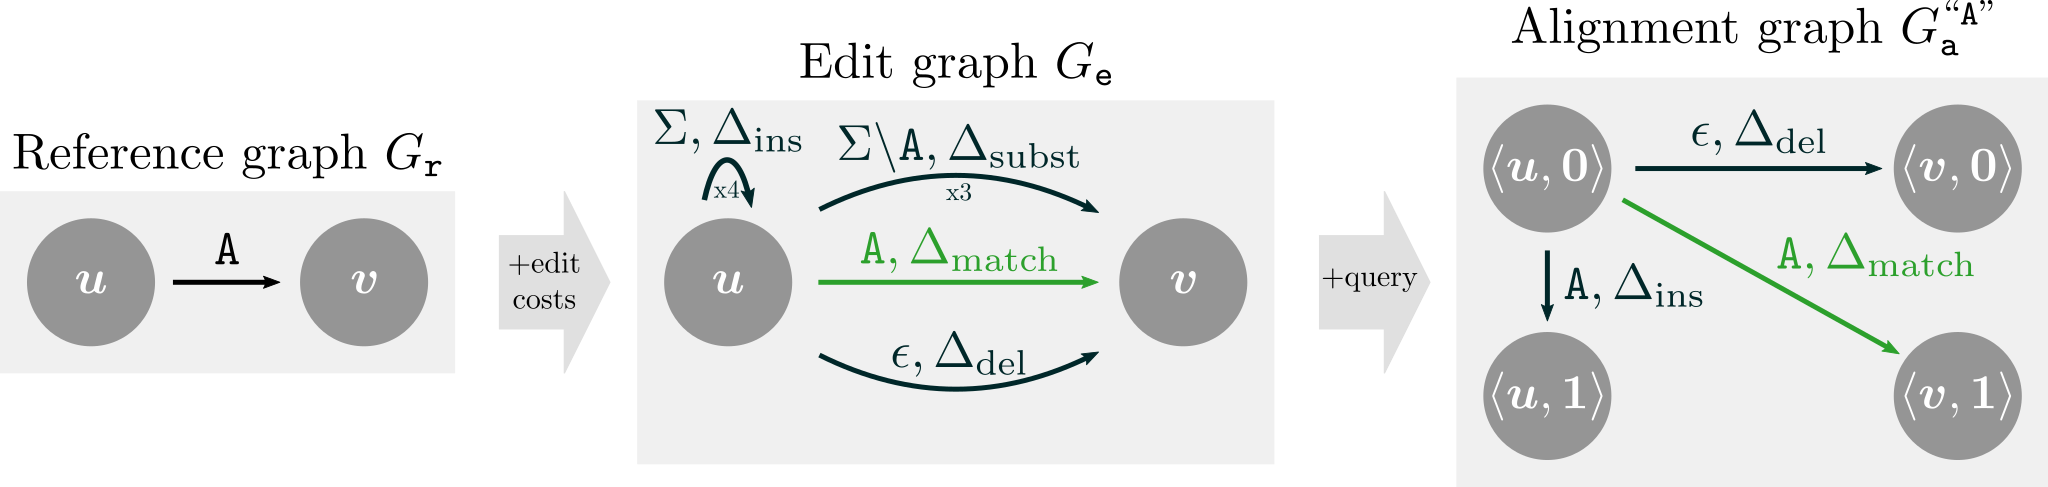
\includegraphics[width=0.8\columnwidth]{edit_graph}
	\caption[Constructing the alignment graph]{Starting from the reference graph (left), we can construct the edit graph (middle) and the alignment graph $\AG$ for query $q=``\texttt{A}"$ (right). Edges are annotated with labels and/or costs, where sets of labels represent multiple edges, one for each letter in the set (indicated by $``\text{x}3"$ and $``\text{x}4"$).}
	\label{TRIEfig:graph-constructions}
\end{figure}

\para{Edit graph}
Instead of representing alignments as pairs of (i)~paths in the reference graph and
(ii)~sequences of edit operations on these paths, we introduce \textit{edit
graphs} whose paths intrinsically capture both. This way, we can
formally define an alignment more conveniently as a path in an edit graph.

Formally, an \emph{edit graph} $\EG:=(\EGV,\EGE)$ has directed, labeled edges
$\EGE \subseteq \EGV \times \EGV \times \Sigma_\epsilon \times \mathbb{R}_{\geq
0}$ with associated costs that account for edits. Here, $\Sigma_\epsilon :=
\Sigma \cup \{\epsilon\}$ extends the alphabet $\Sigma$ by $\epsilon$ to account
for deleted characters (see \cref{TRIEfig:graph-constructions}).
%
The edit and reference graphs consist
of the same vertices, \ie, $\EGV=\RGV$. However, $\EGE$ contains more edges
than $\RGE$ to account for edits.
%
Concretely, for each edge $(u,v,\ell) \in \RGE$, $\EGE$ contains edges to
account for (i)~matches, by an edge $(u,v,\ell,\cmatch)$, (ii)~substitutions, by
edges $(u,v,\ell',\csubst)$ for each $\ell' \in \Sigma \backslash \ell$,
(iii)~deletions, by an edge $(u,v,\epsilon,\cdel)$, and (iv)~insertions, by
edges $(u,u,\ell',\cins)$ for each $\ell' \in \Sigma$.
%
The spelling $\sigma(\pi) \in \Sigma^*$ of a path $\pi \in \EG$ is defined
analogously to reference graphs, except that deleted letters (represented by
$\epsilon$) are ignored. The cost $\cost{\pi}$ of a path $\pi \in \EG$ is the
sum of all its edge costs.

\para{Alignment on edit Graph}
An \emph{alignment} of query $q$ to $\RG$ is a path $\pi \text{ in } \EG$
spelling $q$, \ie, $q=\sigma(\pi)$. An \emph{optimal alignment} is an alignment
of minimal cost.

\para{Alignment graph}
To find an optimal alignment of $q$ to the edit graph $\EG$ using shortest path
finding algorithms, we must ensure that only paths spelling $q$ are considered.
To this end, we introduce an alternative but equivalent formulation of
alignments in terms of an \emph{alignment graph} $\AG=(\AGV,\AGE)$.

Here, each \emph{state} $\langle v,i \rangle \in \AGV$ consists of a vertex $v \in
\EGV$ and a query position $i \in \{0,\dots,|q|\}$ (equivalent
to~\cite{rautiainen_aligning_2017}). Traversing a state $\langle v,i \rangle \in
\AGV$ represents the alignment of the first $i$ query characters ending at node $v$.
%
In particular, query position $i=0$ indicates that we have not yet matched any
letters from the query.
%
We note that the alignment graph explicitly depends on the query $q$. In
particular, the example alignment graph $\AG[``\texttt{A}"]$ in
~\cref{TRIEfig:graph-constructions} lacks substitution edges from $\EG$, as their
labels ($\texttt{C}$, $\texttt{G}$, $\texttt{T}$) do not match the query
$q=``A"$.

We construct the alignment graph $\AG$ to guarantee that any walk from a source
$\langle u,0 \rangle$ to a state $\langle v,i \rangle$ corresponds to an
alignment of the first $i$ letters of query $q$ to $\RG$. As a consequence,
there is a one-to-one correspondence between alignments $\edit{\pi}$ of $q$ to
$\EG$ and paths $\alignment{\pi} \in \AG$ from sources $S:=\RGV \times \{0\}$ to
targets $T:=\RGV \times \{|q|\}$, with
$\cost{\reference{\pi}}=\cost{\alignment{\pi}}$. To find the best alignment in
$\EG$, only paths in $\AG$ (walks without repeating nodes) can be considered,
since repeating a node in $\AG$ cannot lead to a lower cost ($\cdel \geq 0$) for
the same state.

\begin{samepage}
The edges $\AGE \subseteq \AGV \times \AGV \times \Sigma_\epsilon \times
\mathbb{R}_{\geq 0}$ are built based on the edges in $\EGE$, except that the
former (i)~keep track of the position in the query $i$, and (ii)~only contain
empty edges or edges
whose label matches the next query letter:

\vspace{-1.2em}
{%
\small
\begin{alignat}{10}
	(u,v,\ell,w) &\in \EGE \implies (&\langle u, i \rangle, &\langle v, i+1
		&&\rangle,\ell,w) \in \AGE \quad \text{ for } 0 \leq i < |q| \text{ with }
		q[i]=\ell \label{TRIEeq:alignment-edges-nondeletions} \\
	(u,v,\epsilon,w) &\in\EGE \implies (&\langle u, i \rangle, &\langle v, i
		&&\rangle,\epsilon,w) \in \AGE \quad \text{ for } 0 \leq i < |q| \label{TRIEeq:alignment-edges-deletions}
\end{alignat}
}%
\end{samepage}
%
Here, assuming $0$-indexing, $q[i]$ is the next letter to be matched after
matching $i$ letters. Then, \cref{TRIEeq:alignment-edges-nondeletions} represents
matches, substitutions, and insertions (which advance the position in the query
by $1$), while \cref{TRIEeq:alignment-edges-deletions} represents deletions (which do
not advance the position in the query).

\para{Dynamic construction}
As the size of the alignment graph is $\Oh(\lvert \RG \rvert \concat \lvert q
\rvert)$, it is expensive to build it fully for every new query.
Therefore, our implementation constructs the alignment graph $\AG$ on-the-fly:
the outgoing edges of a node are only generated on demand and are freed from
memory after alignment.
\section{Dynamic programming}


\section{State of the optimal alignment field}

Comparing one sequence to another is a basic combinatorial problem that has
several variations (shown on the right), each applicable in computational
biology. Needleman-Wunsch (1970)  and Smith-Waterman (1981) are dynamic
programming (DP) algorithms that serve as base solutions for global (or
computing edit distance of two strings) and semi-global alignments (or mapping
when a set of sequences is being aligned). Given that there is both biological
and technical variation in the data, a biologically plausible alignment is one
that minimizes the corresponding differences (e.g. insertions, deletions and
substitutions), so metrics based on edit distance are usually used. Backurs and
Indyk (2015) showed that even calculating the edit distance between two
sequences (without finding an alignment), is not generally solvable in
strongly-subquadratic time. Moreover, even for related sequences of lengths n
and m and edit distance s, the fastest optimal global (Marco-Sola et al., 2021;
Šošic and Šikic, 2017)) and semi-global aligners (Rautiainen et al., 2017) scale
quadratically when the edit distance increases with the length, which is the
case for sequencing errors and biological variation: O(s*min(n,m))=O(enm) and
O(nm), respectively, where e is the error rate (Navarro, 2001). In the age of
big data and long reads (e.g. PacBio, ONP), this quadratic scaling with length
is prohibitive, so the algorithms with practical usage (e.g. minimap2, bwt,
kallisto) do not guarantee optimality but run in subquadratic time (Kucherov,
2019). The gap between fast and optimal global alignment has been recognized but
no optimal algorithms are known that run subquadratically for related sequences
(Medvedev, 2022a). The interest towards genome graphs keeps increasing with the
first International Genome Graph Symposium being held this year in Ascona,
Switzerland (2022). The benefits of using graph references representing
biological variation has been demonstrated to increase the alignment quality
(Garrison et al., 2018). The transition towards graph references only aggravates
the computational issues owing to the potentially complex graph topology (Equi
et al., 2019). The optimal algorithms used in computational biology explore the
search space of possible alignments in an uninformed fashion: by aligning a
prefix of one sequence to a prefix of the other. This contrasts with the
informed search algorithms such as the algorithm by Hunt and Szymanski (1977)
solving the longest common subsequence (LCS) problem (a special case of the edit
distance alignment). Sequence alignment can naturally be formulated as a
shortest path problem solvable by Dijkstra’s algorithm (Ukkonen, 1985). A* is an
informed generalization of Dijkstra’s algorithm (Hart, 1968) but it has not been
successfully applied to sequence alignment. A* may be the missing piece in the
“a major open problem to implement an algorithm with linear-like empirical
scaling on inputs where the edit distance is linear in n” (Medvedev, 2022a).

\subsection{Semi-global alignment (Mapping)}

\begin{floatingfigure}[l]{0.5\textwidth}
    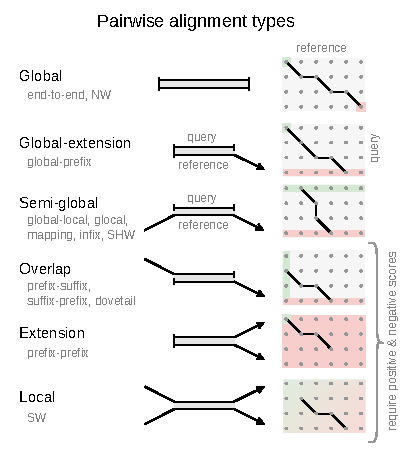
\includegraphics[width=0.5\textwidth]{alignment-types}
	\caption[Alignment types]{Alignment types.}
    \label{fig:alignment-types}
\end{floatingfigure}

% paper-trie; seed-and-extend approach to semi-global alignment
\paragraph{Seed-and-Extend}
Since optimal alignment is often intractable, many aligners use heuristics, most
commonly the \emph{seed-and-extend}
paradigm~\cite{altschul_basic_1990,langmead_fast_2012,li_fast_2009}. In this
approach, alignment initiation sites (\emph{seeds}) are determined, which are
then \emph{extended} to form the \emph{alignments} of the query sequence. The
fundamental issue with this approach, however, is that the seeding and extension
phases are mostly decoupled during alignment. Thus, an algorithm with a provably
optimal extension phase may not result in optimal alignments due to the
selection of a suboptimal seed in the first phase. In cases of high sequence
variability, the seeding phase may even fail to find an appropriate seed from
which to extend.

%%%%%%%%%%%%%%%%%%%%%%%%%%%%%%%%%
%\subsection{Related work}

% Brownie aligner
BrownieAligner, another recent work developed for local alignment of sequences
to {\itshape de Bruijn} graph representations of genomic variation, features an
optimal extension phase using a branch-and-bound-based early cutoff, while
employing a heuristic maximal-exact-match approach for
seeding~\cite{heydari_browniealigner_2018}.
\section{Global alignment}

\subsection{Pangenomes and reference graphs}

The shortest path approach naturally fits more complex references than linear.
In fact, any graph reference (incl. cycles) is fine.

% paper-trie; Accounting for variation
%\para{Accounting for Variation}
First attempts to include variation into the reference data structure were made
by augmenting the local alignment method to consider alternative walks during the
extend step~\cite{schneeberger_simultaneous_2009,palmapper}. This approach has
since been extended from the linear reference case to graph references. To
represent non-reference variation of multiple references during the seeding
stage, HISAT2 uses generalized compressed suffix
arrays~\cite{siren_indexing_2014} to index walks in an augmented reference
sequence, forming a local genome graph~\cite{kim_graphbased_2019}.
VG~\cite{garrison_variation_2018} uses a similar
technique~\cite{siren_indexing_2017} to index variation graphs representing a
population of references.

% paper-trie; The benefit from genome graphs
Historically, a single linear reference sequence has been used to represent the
most common variants in a population. While providing a working abstraction for
most cases, rare or sub-population specific variation is especially hard to
model in this setting, creating a reference allele
bias~\cite{stevenson_sources_2013,brandt_mapping_2015}. Consequently, in the
last few years, the field has shifted first towards using sets of reference
sequences, and more recently to graph data structures (so-called {\em genome
graphs}), to represent many genomes or haplotypes
simultaneously~\cite{dilthey_improved_2015,paten_genome_2017,garrison_variation_2018}.
\input{\dir/shortestpath}
\section{\A algorithm and its heuristic function} \label{sec:astar}

% paper: trie
\subsection{Background: General \A algorithm} \label{TRIEsubsec:general-astar}
Given a weighted graph $G=(V,E)$ with $E \subseteq V \times V \times
\mathbb{R}_{\geq 0}$, the \A algorithm (abbreviated as \A) searches for the
shortest path from sources $S \subseteq V$ to targets $T \subseteq V$. It is an
extension of \dijkstra's algorithm that additionally leverages a \emph{heuristic
function} $h \colon V \to \mathbb{R}_{\geq 0}$ to decide which paths to explore
first.
%
If $h(u) \equiv 0$, \A is equivalent to \dijkstra's algorithm.
%
You can refer to the \A and \dijkstra algorithms in \cref{alg:astar}, but do not
assume knowledge of either algorithm in the following.
%
At a high level, \A maintains the set of all \emph{explored} states, initialized
with the set of sources $S$. Then, \A iteratively \emph{expands} the explored
state with lowest estimated cost by exploring all its neighbors, until it finds
a target. Here, the cost for node $u$ is estimated by the distance from source, called $g(u)$, plus the estimate from the heuristic $h(u)$.

\para{Heuristic Function}
The heuristic function $h(u)$ estimates the
cost $h^*(u)$ of a shortest path in $G$ from $u$ to a target $t \in T$. Intuitively, a
good heuristic correlates well with the distance from $u$ to $t$.

To ensure that \A indeed finds the shortest path, $h$ should be
\emph{admissible}:

\begin{definition}[Admissible heuristic] A heuristic $h$ is \emph{admissible}
    if it provides a lower bound on the distance to the closest target: $\forall
    u. h(u) \leq h^*(u)$.
\end{definition}

While any admissible $h$ ensures that \A finds optimal
alignments~\cite{dechter_generalized_1985}, the specific choice of $h$
is critical for performance. In particular, decreasing the error $\delta(u) =
h^*(u)-h(u)$ can only improve the performance of
\A~\cite{dechter_generalized_1985}. Thus, a key contribution of ours is
a domain-specific heuristic $h$.


\para{\A algorithm}
We aim to guarantee optimal alignment while optimizing the average runtime
to not reach its worst-case complexity. While \dijkstra is an algorithm that
explores graph nodes in the order of their distance from the start, \A is a
generalization of \dijkstra that also accounts for their distance from the
target. \A prioritizes the exploration of nodes that seem to be closer to the
target nodes. This way, \A can sometimes dramatically improve on the performance
of \dijkstra while remaining optimal.

There has been one attempt to apply \A for optimal
alignment~\cite{dox2018efficient} which uses a heuristic function that accounts
only for the length of the remaining query sequence to be aligned. However, it
does not significantly outperform \dijkstra (in fact, it is equivalent for
a zero matching cost).
%
In contrast, the heuristic function we introduce is more informative and
consistently outperforms \dijkstra.

\cref{alg:astar} shows a generic implementation of the \A algorithm,
roughly following~\cite{dechter_generalized_1985}.
We do not implement the reconstruction of the best alignment in order to simplify the presentation.
The procedure \mbox{\textsc{BacktrackPath}} traces the best alignment back to the $source$, based on remembered edges used to optimize $f$ for each alignment state.
%
\cref{alg:astar} also shows a simple implementation of \dijkstra in terms of \A.
We omit the implementation of \textsc{BacktrackPath} for simplicity.

\begin{algorithm}[t]
	\caption{\A~algorithm} \label{alg:astar}
	\begin{algorithmic}[1]
		\Function{\A}{$G\colon \text{Graph}$,
			$S\colon \text{Sources}$,
			$T\colon \text{Targets}$,
			$h\colon \text{Heuristic function}$}
		\State $g \gets \mli{Map}\colon (\text{Nodes} \to \mathbb{R}_{\geq 0})$
		\Comment Shortest paths lengths to explored nodes

		\State $f \gets \mli{Map}\colon (\text{Nodes} \to \mathbb{R}_{\geq 0})$
		\Comment $f(u)=g(u)+h(u)$ 

		\State $Q \gets \mli{MinPriorityQueue}(\mli{priority}=f)$ 
		\Comment Priorities according to $f$
		\ForAll{$s \in S$}
			\State $g[s] \gets 0.0,\, f[s] \gets 0.0$
			\State $Q.\mli{push}(s)$
			\Comment Initially, explore all $s \in S$
		\EndFor
		\While{$Q \neq \emptyset$}
			\State $\mli{curr} \gets Q.\mli{pop}()$
			\Comment Get state with minimal $f$ to be expanded
			\If{$\mli{curr} \in T$}
				\State \Return \Call{BacktrackPath}{$\mli{curr}$}
				\Comment Reconstruct a walk to $\mli{curr}$
			\EndIf
			\ForAll{$(\mli{curr},\mli{next},\mli{cost}) \in G.\mli{outgoingEdges}(\mli{curr})$}
			\State $g_\mli{next} \gets g[\mli{curr}] + \mli{cost}$
			\State $\hat{f}_\mli{next} \gets g_\mli{next} + h(\mli{next})$
				\Comment Candidate value for $f[\mli{next}]$
				\If{$\hat{f}_\mli{next} < f[\mli{next}{}]$}
					\State $g[\mli{next}] \gets g_\mli{next}$		
					\State $f[\mli{next}] \gets \hat{f}_\mli{next}$		
					\State $Q.\mli{push}(\mli{next})$
					\Comment Explore state $\mli{next}$
				\EndIf
		\EndFor
		\EndWhile
		\State \textbf{assert} $\mli{False}$
		\Comment Cannot happen if $T$ is reachable from $S$
		\EndFunction

		\Statex

		\Function{\dijkstra}{$G\colon \mli{Graph}$,
			$S\colon \mli{Sources}$,
			$T\colon \mli{Targets}$}
			\State $h(v) \gets 0.0$
			\Comment Constant-zero function $h$
			\State $\Call{\A}{G,S,T,h}$
		\EndFunction
	\end{algorithmic}
\end{algorithm}

% paper: seeds

\subsection{\A~algorithm for finding a shortest path} \label{SEEDsec:astar}
%
The \A~algorithm is a shortest path algorithm that generalizes \dijkstra's
algorithm by directing the search towards the target.
Given a weighted graph $G=(V,E)$, the \A~algorithm finds a shortest path from
sources $S \subseteq V$ to targets $T \subseteq V$.
%
To prioritize paths that lead to a target, it relies on an admissible heuristic
function $h \colon V \to \mathbb{R}_{\geq 0}$, where $h(v)$ estimates the
remaining length of the shortest path from a given node $v \in V$ to a target
$t \in T$.


\para{Algorithm}
% 
In a nutshell, the \A~algorithm maintains a set of \emph{explored} nodes,
initialized by all possible starting nodes $S$. It then iteratively
\emph{expands} the explored state $v$ with lowest estimated total cost $f(v)$ by
exploring all its neighbors. Here, $f(v) := g(v) + h(v)$, where $g(v)$ is the
distance from $s \in S$ to $v$, and $h(v)$ is the estimated distance from $v$ to
$t \in T$.
%
When the \A~algorithm expands a target node $t \in T$, it reconstructs the path
leading to $t$ and returns it.
%
For completeness, \cref{SEEDapp:astar} provides an implementation of \A.

\para{Admissibility}
%
The \A~algorithm is guaranteed to find a shortest path if its heuristic $h$
provides a lower bound on the distance to the closest target, often referred to
as $h$ being \emph{admissible} or optimistic.

Further, the performance of the \A~algorithm relies critically on the choice of
$h$. Specifically, it is crucial to have low estimates for the optimal paths but
also to have high estimates for suboptimal paths.

\para{Discussion}
%
To summarize, we use the \A~algorithm to find a shortest path from $\st{u}{0}$
to $\st{v}{|q|}$ in $\AG$. To guarantee optimality, its heuristic function
$h\st{v}{i}$ must provide a lower bound on the shortest distance from state
$\st{v}{i}$ to a terminal state of the form $\st{w}{\lvert q \rvert}$.
%
Equivalently, $h\st{v}{i}$ should lower bound the minimal cost of aligning
$q[i{:}]$ to $\RG$ starting from $v$, where $q[i{:}]$ denotes the suffix of $q$
starting at position $i$ ($0$-indexed).
%
The key challenge is thus finding a heuristic that is not only admissible but
also yields favorable performance.

% paper:global
% Shortest paths, A* for MSA and semi-global alignment (AStarix), gaps
\paragraph{Shortest paths and \A}
A pairwise alignment that minimizes edit distance corresponds to a shortest path in the
\emph{edit graph}~\citep{vintsyuk1968speech,ukkonen1985algorithms}. Assuming
non-negative edit costs, a shortest path can be found using \dijkstra's
algorithm~\citep{ukkonen1985algorithms} (\cref{GLOBALfig1-dij}) or
\A~\citep{spouge1989speeding}. \A is an informed search algorithm which uses a
task-specific heuristic function to direct its search. Depending on the
heuristic function, a shortest path may be found significantly faster than by an
uninformed search such as \dijkstra's algorithm. In the context of semi-global
sequence-to-graph alignment, \A has been used to empirically scale sublinearly
with the reference size for short reads~\citep{ivanov2020astarix}.
% paper: global
\paragraph{Seeds, and matches}

Seed-and-extend is a commonly used paradigm for solving semi-global
alignment approximately~\citep{kucherov2019evolution}.
Seeds are also used to define and compute LCSk~\citep{benson2014longest}, a
generalization of longest common subsequence (LCS). In contrast, the \emph{\sh}
by~\citet{ivanov2022fast} speeds up finding an optimal alignment by
using seed matches to speed up the \A search. The \sh enables
empirical near-linear scaling to long HiFi reads (up to $30\kbp$ with $0.3\%$
errors)~\citep{ivanov2022fast}. A limitation of the existing \sh is the low
tolerance to increasing error rates due to using only long exact matches without
accounting for their order.
\section{Contributions}

\paragraph{Tools}

\subsection{Informed search}
Two-stage algorithm, similar to Aho-Corasick, increasingly more information (length, prefix, seeds, chaining seeds, chaining seeds + gaps)
 
% Accuracy and Metrics
The number of possible alignments grow exponentially with length. The usual
underlying question to finding ``correct'' alignments. Regarding the precision
of alignment, one is usually interested in base-to-base (aka letter-to-letter)
correspondence between the sequences, even though for some applications a less
detailed solution is sufficient: only the similarity between sequences or the
location where a read maps to a reference. Exact alignment is only useful for
very short sequences (often kmers), and for all other cases the optimized metric
may be hamming distance, edit distance (unit costs), Levenshtein distance,
affine costs, convex and concave costs, general costs and others. 

% Problem statement
Depending on the the number of aligned sequences, there is pairwise alignment
and multiple sequence alignment (MSA). Depending on the parts of the sequences
that are aligned to each other, we differentiate global, local and various
semi-global alignemnts. There are generalizations to sequence-to-sequence
alignment, including aligning to nonlinear structures, such as directed acyclic
graphs, DAGs, general graphs and others. These structures are nowadays becoming
more common as a compressed form of representing a set of references to which a
sequence can be aligned. Often, one best alignment is suefficient but finding
several best (top-K) alignments. In the context of read mapping, a set of reads
is aligned to the same reference sequence so an indexing procedure is often
useful for the performance.

We specifically consider the mapping of a set of reads to a general graph, and
the global pairwise alignment.

Existing optimal algorithms are based on dynamic programming (DP) and
run in quadratic time (assuming that the number of errors is proportional to the
length)

we employ the \A algorithm which is an \emph{informed search} algorithm.
TODO: a case for the informed algorithms

\subsection{Scalable optimal alignments}

% Heuristics for alignment
Both for sequence-to-sequence alignment and sequence-to-graph alignment,
heuristics are employed to keep alignment
tractable~\cite{altschul_basic_1990,langmead_fast_2012,garrison_variation_2018},
especially for large populations of human-sized genomes.
%
% Importance of optimal alignment
While such heuristics find the correct alignment for simple references, they
often perform poorly in regions of very high complexity, such as in the human
major histocompatibility complex (MHC)~\cite{dilthey_improved_2015}, in complex
but rare genotypes arising from somatic-subclones in tumor sequencing
data~\cite{harismendy_detection_2011}, or in the presence of frequent sequencing
errors~\cite{salmela_lordec_2014}.
%
Importantly, these cases can be of specific clinical or biological interest, and
incorrect alignment can cause severe biases for downstream analyses. For
instance, the combination of high variability of MHC sequences in humans and
small differences between alleles~\cite{buhler_hla_2011} leads to a risk of
misclassifications due to suboptimal alignment. Guaranteeing optimal alignment
against all variations represented in a graph is a major step towards
alleviating those biases.

% Optimal DP-based approaches
\paragraph{Optimal Alignment}
Current optimal alignment algorithms reach the impractical $\Oh(nm)$ runtime
that has been shown to be a lower bound for the worst-case edit distance
computation~\cite{backurs2015edit}. In this light, approaches for improving the
efficiency of optimal alignment have taken advantage of specialized features of
modern CPUs to improve the practical runtime of the Smith-Waterman dynamic
programming (DP) algorithm~\cite{smith_comparison_1981} considering all possible
starting nodes. These use modern SIMD instructions (\eg
\vg~\cite{garrison_variation_2018} and \pasgal~\cite{jain_accelerating_2019}) or
reformulations of edit distance computation to allow for bit-parallel
computations in \graphaligner \footnote{We refer as \bitparallel to to the
bit-parallel DP algorithm implemented in \graphaligner tool
\cite{rautiainen_bitparallel_2019}.}~\cite{rautiainen_bitparallel_2019}. Many of
these, however, are designed only for specific types of genome graphs, such as
{\itshape de Bruijn}
graphs~\cite{liu_debga_2016,limasset2019toward} and
variation graphs~\cite{garrison_variation_2018}. A compromise often made when
aligning sequences to cyclic graphs using algorithms reliant on directed acyclic
graphs involves the computationally expensive ``DAG-ification'' of graph
regions~\cite{kavya_sequence_2019,garrison_variation_2018}.

%\section{Optimal alignment}
Finding an optimal alignment requires a conceptually different approach than
finding an approximate alignment. Instead of finding \emph{one} good alignment,
finding an optimal alignment requires proving that \emph{all} other
exponentially-many alignments are not better.

Comparing one sequence to another is a basic combinatorial problem that has
several variations (shown on the right), each applicable in computational
biology. Needleman-Wunsch (1970)  and Smith-Waterman (1981) are dynamic
programming (DP) algorithms that serve as base solutions for global (or
computing edit distance of two strings) and semi-global alignments (or mapping
when a set of sequences is being aligned). Given that there is both biological
and technical variation in the data, a biologically plausible alignment is one
that minimizes the corresponding differences (e.g. insertions, deletions and
substitutions), so metrics based on edit distance are usually used. Backurs and
Indyk (2015) showed that even calculating the edit distance between two
sequences (without finding an alignment), is not generally solvable in
strongly-subquadratic time. Moreover, even for related sequences of lengths n
and m and edit distance s, the fastest optimal global (Marco-Sola et al., 2021;
Šošic and Šikic, 2017)) and semi-global aligners (Rautiainen et al., 2017) scale
quadratically when the edit distance increases with the length, which is the
case for sequencing errors and biological variation: O(s*min(n,m))=O(enm) and
O(nm), respectively, where e is the error rate (Navarro, 2001). In the age of
big data and long reads (e.g. PacBio, ONP), this quadratic scaling with length
is prohibitive, so the algorithms with practical usage (e.g. minimap2, bwt,
kallisto) do not guarantee optimality but run in subquadratic time (Kucherov,
2019). The gap between fast and optimal global alignment has been recognized but
no optimal algorithms are known that run subquadratically for related sequences
(Medvedev, 2022a). The interest towards genome graphs keeps increasing with the
first International Genome Graph Symposium being held this year in Ascona,
Switzerland (2022). The benefits of using graph references representing
biological variation has been demonstrated to increase the alignment quality
(Garrison et al., 2018). The transition towards graph references only aggravates
the computational issues owing to the potentially complex graph topology (Equi
et al., 2019). The optimal algorithms used in computational biology explore the
search space of possible alignments in an uninformed fashion: by aligning a
prefix of one sequence to a prefix of the other. This contrasts with the
informed search algorithms such as the algorithm by Hunt and Szymanski (1977)
solving the longest common subsequence (LCS) problem (a special case of the edit
distance alignment). Sequence alignment can naturally be formulated as a
shortest path problem solvable by Dijkstra’s algorithm (Ukkonen, 1985). \A is an
informed generalization of Dijkstra’s algorithm (Hart, 1968) but it has not been
successfully applied to sequence alignment. \A may be the missing piece in the
“a major open problem to implement an algorithm with linear-like empirical
scaling on inputs where the edit distance is linear in n” (Medvedev, 2022a).
